\documentclass[14pt, aspectratio=169]{beamer}
\usepackage{unicode}
\usepackage[notocbib]{apacite}
\usepackage{parskip}
\usepackage{times}
\usepackage{tabularx}
\usepackage{tikz}
\usepackage{mdframed}
\usepackage{caption}
\usepackage{xcolor}
\usepackage{pifont}

\renewcommand{\bibname}{Referencias Bibliográficas}
\renewcommand{\contentsname}{Tabla de Contenido}
\renewcommand{\chaptername}{Capítulo}
\renewcommand{\figurename}{Figura}
\renewcommand{\tablename}{Tabla}


\newcommand {\scaledimage}[1] {
    \includegraphics[width=\textwidth,height=0.8\textheight,keepaspectratio]{#1}
}
\usetikzlibrary{positioning,arrows,automata}
\setbeamertemplate{navigation symbols}{}

\title{Especificación del Analizador Léxico}
\author{Aramis E. Matos, Lenier Gerena, Angel Berrios}
\date{2/28/2023}

\usetheme{Berlin}
\usecolortheme{beaver}
\setbeamertemplate{headline}{}

\begin{document}
\maketitle

\begin{frame}[allowframebreaks]
    \frametitle{Índice}
    \tableofcontents
\end{frame}

\section{Introduccion}

\begin{frame}{Introduccion}
    \cite{narciso_farias_gramatica_2012}

    \cite{tapkeer_flex_2023}
\end{frame}

\section{Gramatica de AVISMO}

\begin{frame}[allowframebreaks]
    \frametitle{Gramatica de AVISMO}
    \begin{itemize}
        \item $<$SENTENCIAS$>$ ::= <FIN\_DE\_LINEA> $<$SENTENCIAS$>$ | $<$SENTENCIA$>$ $<$FIN\_DE\_LINEA$>$
        \item $<$FIN\_DE\_LINEA$>$ ::= ":" | ";"
        \item $<$SENTENCIA$>$ ::= "defina" $<$ID$>$ "como" $<$TIPO$>$ | $<$ID$>$ "="  $<$MODELO\_MOLECULAR$>$ | $<$OPERACION$>$ "(" $<$ID$>$ ")"
        \item $<$ID$>$ ::= "A" | "B" | "C" | "D" | "E" | "F" | "G" | "H" | "I" | "J" | "K" | "L" | "M" | "N" | "O" | "P" | "Q" | "R" | "S" | "T" | "U" | "V" | "W" | "X" | "Y" | "Z" | "a" | "b" | "c" | "d" | "e" | "f" | "g" | "h" | "i" | "j" | "k" | "l" | "m" | "n" | "o" | "p" | "q" | "r" | "s" | "t" | "u" | "v" | "w" | "x" | "y" | "z" | $<$LETRA$>$ $<$IDCONT$>$
        \item $<$IDCONT$>$ ::= "A" | "B" | "C" | "D" | "E" | "F" | "G" | "H" | "I" | "J" | "K" | "L" | "M" | "N" | "O" | "P" | "Q" | "R" | "S" | "T" | "U" | "V" | "W" | "X" | "Y" | "Z" | "a" | "b" | "c" | "d" | "e" | "f" | "g" | "h" | "i" | "j" | "k" | "l" | "m" | "n" | "o" | "p" | "q" | "r" | "s" | "t" | "u" | "v" | "w" | "x" | "y" | "z" | $<$LETRA$>$ $<$IDCONT$>$ | "0" | "1" | "2" | "3" | "4" | "5" | "6" | "7" | "8" | "9" | $<$DIGITO$>$ $<$IDCONT$>$
        \item $<$LETRA$>$ ::= "A" | "B" | "C" | "D" | "E" | "F" | "G" | "H" | "I" | "J" | "K" | "L" | "M" | "N" | "O" | "P" | "Q" | "R" | "S" | "T" | "U" | "V" | "W" | "X" | "Y" | "Z" | "a" | "b" | "c" | "d" | "e" | "f" | "g" | "h" | "i" | "j" | "k" | "l" | "m" | "n" | "o" | "p" | "q" | "r" | "s" | "t" | "u" | "v" | "w" | "x" | "y" | "z"
    \end{itemize}
\end{frame}

\section{Especificación del Analizador Léxico}

\begin{frame}{Especificación del Analizador Léxico}
    \only<1> {
        \begin{table}[ht]
            \footnotesize
            \begin{tabularx}{\linewidth}{|X|X|X|}
                \hline
                \textit{Token}        & Patrones                                                                  & Atributos                                         \\\hline
                <FIN\_DE\_ LINEA>     & ; | :                                                                     & Indica fin de Línea                               \\\hline
                <PALABRA\_ RESERVADA> & defina | como                                                             & Indica declaración de una variable                \\\hline
                <ID>                  & [A-Za-z] | <LETRA> <IDCONT>                                               & Apuntador a la tabla de símbolos                  \\\hline
                <IDCONT>              & \textit{[A-Za-z]} | <LETRA> <IDCONT> | \textit{[0-9]} | <DIGITO> <IDCONT> & Permite que los identificadores contengan números \\\hline
            \end{tabularx}
            \label{table: lexTable1}
            \caption{Definición Léxica del Lenguaje AVISMO}
        \end{table}
    }
    \only<2> {
        \begin{table}[ht]
            \footnotesize
            \begin{tabularx}{\linewidth}{|X|X|X|}
                \hline
                \textit{Token} & Patrones                    & Atributos                                       \\\hline
                <ASIGNACION>   & =                           & Asigna un <MODELO\_MOLECULAR a un identificador \\\hline
                <ID>           & [A-Za-z] | <LETRA> <IDCONT> & Indica declaración de una variable              \\\hline
                <LETRA>        & [A-Za-z]                    & Provee un terminal para <ID> y <IDCONT>         \\\hline
                <DIGITO>       & [0-9]                       & Escribir algo                                   \\\hline
            \end{tabularx}
            \label{table: lexTable2}
            \caption{Definición Léxica del Lenguaje AVISMO}
        \end{table}
    }
\end{frame}

\section{Diseño del Analizador Léxico}

\subsection{Autómatas Finitos Deterministas}

\begin{frame}{Diseño del Analizador Léxico}
    \only<1>{
        \begin{figure}[ht]
            \footnotesize
            \begin{minipage}{.4\textwidth}
                \centering
                \begin{mdframed}
                    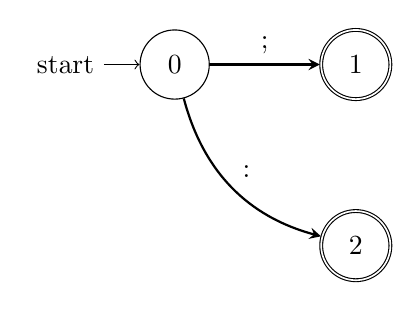
\begin{tikzpicture}[node distance = 2.3cm, on grid, auto]
                        \node [state,initial] (q0) {$0$};
                        \node [state,accepting] [right=of q0] (q1) {$1$};
                        \node [state,accepting] [below=of q1] (q2) {$2$};

                        \path[-stealth, thick]
                        (q0) edge node {;} (q1)
                        (q0) edge [bend right] node {:} (q2);
                    \end{tikzpicture}
                    \label{fig: finDeLineaAutomata}
                \end{mdframed}
                \caption{Automata del patrón para el token <FIN\_DE\_LINEA>}
            \end{minipage}\hspace{1cm}
            \begin{minipage}{0.4\textwidth}
                \centering
                \begin{mdframed}
                    \begin{tikzpicture}[node distance = 2.3cm, on grid, auto]
                        \node [state, initial] (q0) {$0$};
                        \node [state, accepting] [right=of q0] (q1) {$1$};
                        \node [state, accepting] [below=of q1] {$1$};

                        \path[-stealth, thick]
                        (q0) edge node {defina} (q1)
                        (q0) edge [bend right] node {como} (q2);
                    \end{tikzpicture}
                \end{mdframed}
                \label{fig: palabraReservada}
                \captionof{figure}{Automata del patrón para el token <PALABRAS\_RESERVADA>}
            \end{minipage}
        \end{figure}
    }
    \only<2>{
        \begin{figure}[ht]
            \footnotesize
            \begin{minipage}{0.41\textwidth}
                \begin{mdframed}
                    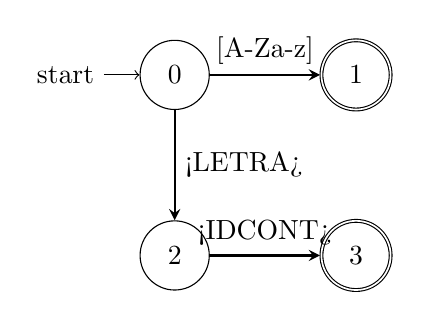
\begin{tikzpicture}[node distance = 1.4cm, auto]
                        \node [state, initial] (q0) {0};
                        \node [state, accepting] [right=of q0] (q1) {$1$};
                        \node [state] [below=of q0] (q2) {$2$};
                        \node [state, accepting] [right=of q2] (q3) {$3$};

                        \path[-stealth, thick]
                        (q0) edge node {[A-Za-z]} (q1)
                        (q0) edge node {<LETRA>} (q2)
                        (q2) edge node {<IDCONT>} (q3);
                    \end{tikzpicture}
                \end{mdframed}
                \label{fig: idAutomata}
                \caption{Automata del patrón para el token <ID>}
            \end{minipage}
        \end{figure}
    }
    \only<3>{
        \begin{figure}[ht]
            \footnotesize
            \begin{minipage}{0.5\textwidth}
                \begin{mdframed}
                    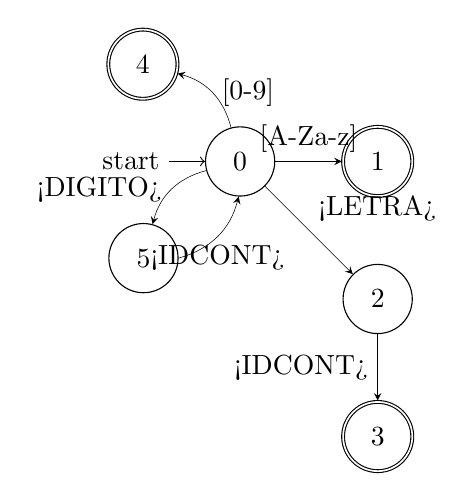
\begin{tikzpicture}[node distance = 24pt,auto]
                        \node [state, initial] (q0) {$0$};
                        \node [state, accepting] [right=of q0] (q1) {$1$};
                        \node [state] [below=of q1] (q2) {$2$};
                        \node [state, accepting] [below=of q2] (q3) {$3$};
                        \node [state, accepting] [above left=of q0] (q4) {$4$};
                        \node [state] [below left=of q0] (q5) {$5$};


                        \path[-stealth, very thin]
                        (q0) edge node {[A-Za-z]} (q1)
                        (q0) edge node {<LETRA>} (q2)
                        (q2) edge node [left] {<IDCONT>} (q3)
                        (q0) edge [bend right] node[right] {[0-9]} (q4)
                        (q0) edge [bend right] node [left] {<DIGITO>} (q5)
                        (q5.east) edge [bend right] node [below] {<IDCONT>} (q0);
                    \end{tikzpicture}
                \end{mdframed}
                \label{fig: idContAutomata}
            \end{minipage} \hspace{1cm}
            \begin{minipage}{0.41\textwidth}
                \caption{Automata del patrón para el token <IDCONT>}
            \end{minipage}
        \end{figure}
    }
    \only<4>{
        \begin{figure}[ht]
            \footnotesize
            \begin{minipage}{0.5\textwidth}
                \begin{mdframed}
                    \begin{tikzpicture}[node distance = 0cm, auto]
                        \node [state,initial] (q0) {$0$};
                        \node [state,accepting] [right=of q1] (q1) {$1$};

                        \path[-stealth,thick]
                        (q0) edge node {=} (q1);
                    \end{tikzpicture}
                \end{mdframed}
                \label{fig: asigAutomata}
                \caption{Automata del patrón para el token <ASIGNACION>}
            \end{minipage}\hspace{1cm}
            \begin{minipage}{0.5\linewidth}
                \begin{mdframed}
                    \begin{tikzpicture}[node distance = 0cm, on grid ,auto]
                        \node [state,initial] (q0) {$0$};
                        \node [state,accepting] [right=of q1] (q1) {$1$};

                        \path[-stealth,thick]
                        (q0) edge node {[0-9]} (q1);
                    \end{tikzpicture}
                \end{mdframed}
                \label{fig: letraAutomata}
                \caption{Automata del patrón para el token <LETRA>}
            \end{minipage}
        \end{figure}
    }
\end{frame}

\subsection{Estructura de Datos de la Tabla de Símbolos}

\begin{frame}
    \frametitle{Estructura de Datos de la Tabla de Símbolos}
    \begin{figure}[H]
        \begin{mdframed}
            \textnormal{var1} $\rightarrow \left\{\textbf{tipo}: \textit{str},\textbf{valor}:\textit{"chungus",\textbf{esMutable} : false}\right\}$

            \textnormal{Big} $\rightarrow \left\{\textbf{tipo}: \textit{int},\textbf{valor}:\textit{"12",\textbf{esMutable} : false}\right\}$
            \begin{center}
                $\vdots$
            \end{center}

            \textit{Identificador}  $\rightarrow \textbf{Atributos de Identificador}$
        \end{mdframed}
        \label{fig: symbolTableStruct}
        \caption{Estructura de la Tabla de Símbolos, un Diccionario}
    \end{figure}
\end{frame}

\begin{frame}{Casos de Prueba}
    \begin{columns}
        \begin{column}{0.5\textwidth}
            {\color{red} \ding{55}} Programas Léxicamente Incorrectos
            \begin{itemize}
                \only<1>{\item incio $\longrightarrow$  Error Léxico\\
                    defina a1 como modelo;
                    a1 = CH3CH(CH3)CH3;
                    fin}
                \only<2>{\item inicio
                    defina a\_1 como modelo; $\longrightarrow$ Error Léxico\\
                    a1 = CH3CH(CH3)CH3;
                    fin}
                \only<3>{\item inicio
                    defina a1 como modelo $\longrightarrow$ Error Léxico\\
                    a1 = CH3CH(CH3)CH3 $\longrightarrow$ Error Léxico\\
                    fin}
            \end{itemize}
        \end{column}

        \begin{column}{0.5\textwidth}
            {\color{green} $\checkmark$} Programas Léxicamente Correctos
            \begin{itemize}
                \only<1>{\item inicio $\longrightarrow$ ID inicio\\
                    defina a1 como modelo;
                    a1 = CH3CH(CH3)CH3;
                    fin}
                \only<2>{\item inicio
                    defina a1 como modelo; $\longrightarrow$ ID a1\\
                    a1 = CH3CH(CH3)CH3;
                    fin}
                \only<3>{\item inicio
                    defina a1 como modelo; $\longrightarrow$ Fin de línea\\
                    a1 = CH3CH(CH3)CH3; $\longrightarrow$ Fin de línea\\
                    fin}
            \end{itemize}
        \end{column}
    \end{columns}
    

\end{frame}
\begin{frame}[allowframebreaks]
    \frametitle{Referencias}
    \bibliography{../../report/References}
    \bibliographystyle{apacite}
\end{frame}


\end{document}
